% Provenance (never printed): old premiere S material on the structure of the
% Earth from seismology (P and S waves, travel times, the Moho, the shadow zone
% and the core, a reference model); see sources/book2/PROVENANCE.md. Profiles
% from figdata/grade-11/prem_profiles.py, rays and travel times from
% seismic_rays.py, the refraction lines and the problem's readings from
% moho_refraction.py. Lehmann's story and portrait are told in Book 1 (g6
% inside-the-earth): recalled here, not repeated.
\chapter{Les ondes sismiques révèlent l'intérieur}\label{ch:g11:seismic-structure}

Le 8~octobre 1909, un séisme secoua la vallée de la Kupa, à environ
\qty{40}{km} au sud-est de Zagreb, en Croatie. Quelques mois plus tôt,
Andrija Mohorovičić avait installé un nouveau sismographe à l'observatoire
météorologique de Zagreb, et l'appareil enregistra tout l'événement. Il
demanda ensuite leurs enregistrements à d'autres observatoires et réunit
ceux de 41 stations. Sur les enregistrements des stations les plus
lointaines, il trouva quelque chose d'inattendu~: deux \omterm{def:g11:seismic-structure:body-waves}{ondes P} distinctes,
une faible puis une plus forte, là où il aurait dû n'y en avoir qu'une. De
cette paire d'ondes, il déduisit que la roche située sous la croûte est
différente, et il mesura la profondeur de la limite. Ce chapitre montre
comment les instants d'arrivée des ondes sismiques révèlent les couches de
la Terre~: la base de la croûte, le noyau et sa partie externe liquide, et
tout l'intérieur, profondeur par profondeur.
% ledger: herak:kupa-1909, srl:mohorovicic, geotech:moho-1909, kayal:pn-sn

\begin{recall}
Un séisme naît en un point situé à l'intérieur de la Terre, le foyer~; le
point de la surface situé juste au-dessus est l'épicentre. Un sismomètre
enregistre les secousses du sol, et la magnitude mesure la taille d'un
séisme (livre~1, année~7). La Terre comprend une croûte, un manteau et un
noyau~; le noyau a une partie externe liquide et une partie interne solide.
Les ondes sismiques sont de deux grands types, les \omterm{def:g11:seismic-structure:body-waves}{ondes P}, plus rapides, et
les \omterm{def:g11:seismic-structure:body-waves}{ondes S}, plus lentes, et les \omterm{def:g11:seismic-structure:body-waves}{ondes S} ne peuvent pas traverser un liquide
(livre~1, année~6). Une onde qui franchit la limite entre deux matériaux
dans lesquels elle se propage aux vitesses $v_1$ et $v_2$ est réfractée~:
$\sin i_1/v_1 = \sin i_2/v_2$, où les angles sont mesurés à partir de la
perpendiculaire à la limite (loi de Snell--Descartes~; les livres de
physique).
\end{recall}

\section{Les ondes sismiques et leurs temps de trajet}

\subsection{Deux sortes d'ondes de volume}

Un séisme envoie des ondes dans toutes les directions. Certaines se
propagent le long de la surface~; d'autres, les ondes de volume, traversent
l'intérieur de la Terre, et ce sont elles qui le révèlent.

\begin{definition}[Onde P~; onde S]\label{def:g11:seismic-structure:body-waves}
Une \emph{onde P}\index{onde P} est une onde sismique qui comprime et étire
alternativement la roche~: la roche va et vient dans la direction de
propagation de l'onde. Elle traverse les solides, les liquides et les gaz,
et c'est l'onde sismique la plus rapide~: elle arrive donc la première. Une
\emph{onde S}\index{onde S} cisaille la roche~: la roche se déplace
perpendiculairement à la direction de propagation de l'onde. Elle ne
traverse que les solides, et elle arrive après l'onde P.
\end{definition}
% ledger: kayal:p-s

Un liquide s'écoule et n'oppose aucune résistance à un changement de forme~:
il ne peut donc pas transmettre un cisaillement. C'est pourquoi les \omterm{def:g11:seismic-structure:body-waves}{ondes S}
s'arrêtent à la surface d'un liquide. Dans la plupart des roches, une \omterm{def:g11:seismic-structure:body-waves}{onde P}
va environ $\sqrt 3 \approx 1.7$ fois plus vite qu'une \omterm{def:g11:seismic-structure:body-waves}{onde S}. Dans la
croûte supérieure, une \omterm{def:g11:seismic-structure:body-waves}{onde P} se propage à environ \qty{5.8}{km/s} et une
\omterm{def:g11:seismic-structure:body-waves}{onde S} à environ \qty{3.2}{km/s}~; juste sous la croûte, elles atteignent
environ \qty{8.1}{km/s} et \qty{4.5}{km/s}.
% ledger: kayal:p-s, kayal:outer-core-liquid, data:prem (vp_surface 5.8, vs_surface 3.2,
% vp_upper_mantle 8.11, vs_upper_mantle 4.49 in figdata/grade-11/prem_profiles.py)

\begin{omfigure}

\includegraphics[width=0.5\linewidth]{images/book2/g11-usgs-seismometer.jpg}

{\small Des sismologues du Puerto Rico Seismic Network et de l'USGS
installent un sismomètre temporaire dans le sud-ouest de Porto Rico, le
10~janvier 2020. Photographie~: Thomas Pratt, USGS (domaine public).}
\end{omfigure}
% ledger: photo:g11-seismometer

\subsection{Les hodochrones}

La distance d'un séisme à une station lointaine se mesure par un angle~:
l'angle $\Delta$, au centre de la Terre, entre l'épicentre et la station,
la \emph{distance épicentrale}\index{distance epicentrale@distance épicentrale}.
Un degré correspond à $\qty{111.2}{km}$ le long de la
surface.
% ledger: earth:Rmean

\begin{definition}[Temps de trajet~; hodochrone]\label{def:g11:seismic-structure:travel-time}
Le \emph{temps de trajet}\index{temps de trajet} d'une onde sismique à une
station est la durée qu'elle met pour aller du foyer à la station.
L'\emph{hodochrone}\index{hodochrone} d'une onde est le graphique de son
temps de trajet en fonction de la distance épicentrale de la station.
\end{definition}

Une station enregistre l'instant où arrive chaque onde~; quand l'instant du
séisme est connu, la différence donne le \omterm{def:g11:seismic-structure:travel-time}{temps de trajet}. Des milliers de
séismes enregistrés par des milliers de stations ont fourni les \omterm{def:g11:seismic-structure:travel-time}{hodochrones}
avec une grande précision. Sur la figure, les courbes sont calculées à
partir du \omterm{def:g11:seismic-structure:reference-model}{modèle de Terre de référence} de la
\cref{sec:g11:seismic-structure:model}, et les points sont des \omterm{def:g11:seismic-structure:travel-time}{temps de
trajet} observés lors de séismes réels~: les deux concordent partout à deux
pour cent près, et le plus souvent à une ou deux secondes près.

\begin{omfigure}
\begin{tikzpicture}
\begin{axis}[omrecord, width=0.84\linewidth, height=6.4cm, xmin=0, xmax=180, ymin=0, ymax=30,
  xtick={0,20,...,180}, ytick={0,5,...,30},
  xlabel={distance épicentrale $\Delta$ (degrés)}, ylabel={temps de trajet (minutes)},
  tick label style={font=\small}, label style={font=\small}, clip=false]
% computed in figdata/grade-11/seismic_rays.py; ledger: data:prem, auspass:surftim
\addplot[omDef, line width=0.9pt] table[x=delta_deg, y=t_min] {figdata/out/grade-11-seismic_rays-ttp.dat};
\addplot[omProp, line width=0.9pt] table[x=delta_deg, y=t_min] {figdata/out/grade-11-seismic_rays-tts.dat};
\addplot[omDef, line width=0.9pt, densely dashed] table[x=delta_deg, y=t_min] {figdata/out/grade-11-seismic_rays-ttpkp.dat};
\addplot[omDef!55, line width=0.9pt, densely dotted] table[x=delta_deg, y=t_min] {figdata/out/grade-11-seismic_rays-ttpkikp.dat};
\addplot[only marks, mark=*, mark size=1.5pt, black] table[x=delta_deg, y=p_min] {figdata/out/grade-11-seismic_rays-observed.dat};
\addplot[only marks, mark=*, mark size=1.5pt, black, unbounded coords=discard] table[x=delta_deg, y=s_min] {figdata/out/grade-11-seismic_rays-observed.dat};
\node[font=\small, text=omProp, anchor=south east] at (axis cs:68,21.2) {S};
\node[font=\small, text=omDef, anchor=north west] at (axis cs:72,11.2) {P};
\node[font=\small, text=omDef, anchor=south, align=center] at (axis cs:158,23.2) {P à travers\\le noyau};
\fill[black!10] (axis cs:98.5,0) rectangle (axis cs:143.8,3.2);
\node[font=\scriptsize, align=center] at (axis cs:121.1,1.6) {pas de P direct};
\end{axis}
\end{tikzpicture}

{\small \omterm{def:g11:seismic-structure:travel-time}{Hodochrones} des \omterm{def:g11:seismic-structure:body-waves}{ondes P} (en bleu) et des \omterm{def:g11:seismic-structure:body-waves}{ondes S} (en orange) d'un
séisme situé en surface, calculées avec le \omterm{def:g11:seismic-structure:reference-model}{modèle de Terre de
référence}~; les courbes en tirets et en pointillés sont des \omterm{def:g11:seismic-structure:body-waves}{ondes P} qui ont
traversé le noyau (pointillés~: le noyau interne). Points noirs~: \omterm{def:g11:seismic-structure:travel-time}{temps de
trajet} observés. Entre environ \ang{99} et \ang{144}, aucune \omterm{def:g11:seismic-structure:body-waves}{onde P}
n'arrive directement (en grisé).}
\end{omfigure}

La courbe des \omterm{def:g11:seismic-structure:body-waves}{ondes S} monte plus fortement que celle des \omterm{def:g11:seismic-structure:body-waves}{ondes P}, si bien
que le délai entre les deux arrivées augmente avec la distance. On obtient
ainsi la distance d'un séisme à partir d'un seul enregistrement.

\begin{method}[Distance d'un séisme d'après le délai S--P]\label{met:g11:seismic-structure:distance}
\begin{enumerate}
  \item Sur l'enregistrement, lire l'instant de la première \omterm{def:g11:seismic-structure:body-waves}{onde P} et celui
        de la première \omterm{def:g11:seismic-structure:body-waves}{onde S}~; leur différence est le délai S--P.
  \item Sur les \omterm{def:g11:seismic-structure:travel-time}{hodochrones} (ou dans une table), chercher la distance
        épicentrale à laquelle la courbe S se trouve au-dessus de la courbe
        P de ce délai.
  \item Convertir en kilomètres, si nécessaire, avec $\qty{111.2}{km}$ par
        degré.
\end{enumerate}
Avec trois stations, l'épicentre est le point situé à la bonne distance des
trois.
\end{method}

\begin{example}[Un séisme à \ang{60}]\label{ex:g11:seismic-structure:sp}
Les \omterm{def:g11:seismic-structure:travel-time}{temps de trajet} observés sont de \qty{608}{s} pour P et de \qty{1101}{s}
pour S à \ang{60}, de \qty{536}{s} et \qty{967}{s} à \ang{50}. Une station
qui enregistre une \omterm{def:g11:seismic-structure:body-waves}{onde S} \qty{493}{s} (8~minutes 13~secondes) après l'\omterm{def:g11:seismic-structure:body-waves}{onde
P} se trouve donc à \ang{60} de l'épicentre~: environ $60 \times 111.2 \approx
\qty{6670}{km}$. À \ang{50}, le délai ne serait que de \qty{431}{s}.
\end{example}
% ledger: auspass:surftim

\begin{omfigure}
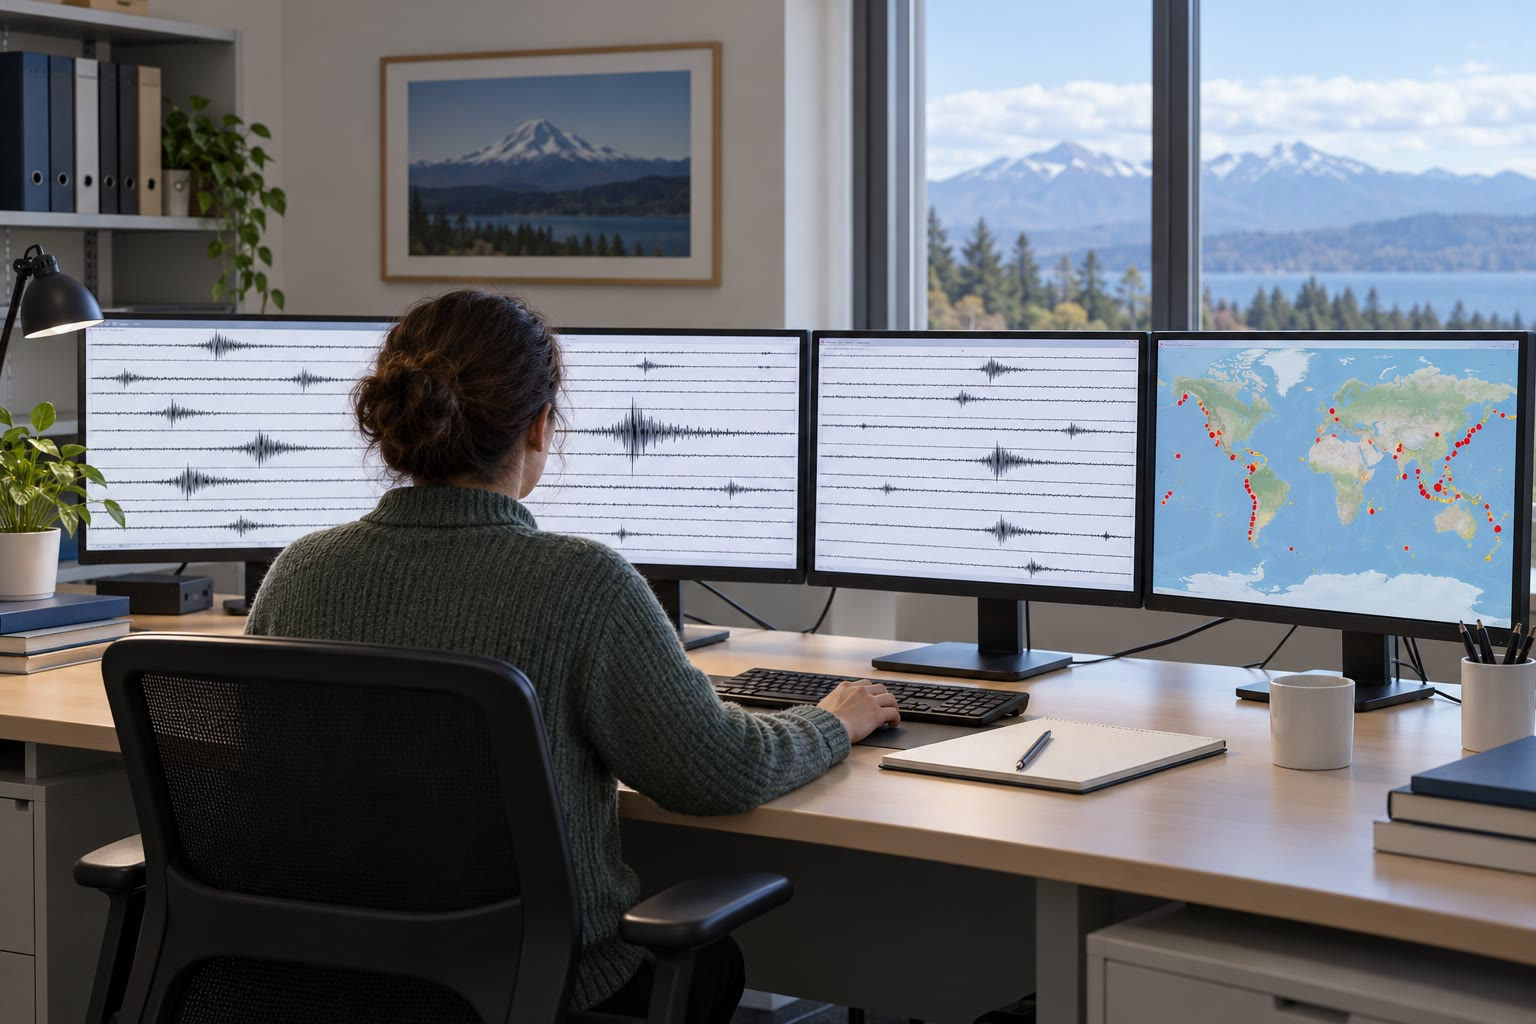
\includegraphics[width=0.66\linewidth]{images/book2/ai/g11-seismology-observatory.jpg}

{\small Dans un observatoire sismologique, les enregistrements de nombreuses
stations sont affichés côte à côte, et les séismes qu'ils permettent de
localiser sont reportés sur une carte du monde (illustration générée par
IA).}
\end{omfigure}

\section{La réfraction et le Moho}\label{sec:g11:seismic-structure:moho}

\subsection{L'onde qui longe une limite}

À l'intérieur de la Terre, la vitesse des ondes sismiques change avec la
profondeur, le plus souvent progressivement, mais par endroits d'un coup.

\begin{definition}[Discontinuité sismique]\label{def:g11:seismic-structure:discontinuity}
Une \emph{discontinuité sismique}\index{discontinuite sismique@discontinuité sismique}
est une surface située à l'intérieur de la Terre à la traversée
de laquelle la vitesse des ondes sismiques change brusquement --- sur une
épaisseur bien plus petite que la longueur des ondes.
\end{definition}

À une discontinuité, une partie de l'onde est réfléchie et une partie est
réfractée. Soit une couche d'épaisseur $h$ dans laquelle les \omterm{def:g11:seismic-structure:body-waves}{ondes P} se
propagent à $v_1$, posée sur une couche où elles sont plus rapides,
$v_2 > v_1$. Un rai qui descend avec l'angle $i$ par rapport à la verticale
est réfracté avec l'angle $r$ donné par $\sin r = (v_2/v_1)\sin
i$~: il s'écarte de la verticale. Quand $\sin i$ atteint $v_1/v_2$, le rai
réfracté longe exactement la limite. L'angle
\[
  i_c, \qquad \sin i_c = \frac{v_1}{v_2},
\]
est l'\emph{angle critique}\index{angle critique}. L'onde réfractée sous
l'\omterm{ex:g11:seismic-structure:sp}{angle critique} se propage le long du sommet de la couche rapide à la
vitesse $v_2$, et, chemin faisant, renvoie des ondes vers le haut dans la
couche supérieure, toutes sous l'angle
$i_c$~: elles atteignent la surface sous la forme de l'\emph{onde
conique}\index{onde conique}.

\begin{omfigure}
\begin{tikzpicture}[x=0.05cm, y=0.05cm, font=\footnotesize, >={Stealth[length=4pt]}]
% geometry from figdata/grade-11/moho_refraction.py: v1 6.2, v2 8.1, h 30 km, ic 49.9 deg
  \fill[omLithGranite!45] (-10,0) rectangle (215,-30);
  \fill[omLithPeridotite!45] (-10,-30) rectangle (215,-48);
  \draw[line width=0.6pt] (-10,0) -- (215,0);
  \draw[line width=0.9pt] (-10,-30) -- (215,-30);
  \node[anchor=west, align=left] at (218,-15) {croûte\\$v_1 = \qty{6.2}{km/s}$};
  \node[anchor=west, align=left] at (218,-39) {manteau\\$v_2 = \qty{8.1}{km/s}$};
  \node[anchor=east] at (215,-26) {Moho};
  % source and station
  \fill[omDef] (0,0) circle (1.6);
  \node[anchor=south] at (0,1.5) {séisme};
  \draw[fill=white] (197,0) -- (203,0) -- (200,5) -- cycle;
  \node[anchor=south] at (200,5) {station};
  % direct wave
  \draw[->, omProp, line width=0.8pt] (2,-2) -- (196,-2);
  \node[anchor=south, text=omProp] at (100,0.3) {onde directe, vitesse $v_1$};
  % head wave
  \draw[omDef, line width=0.9pt] (0,0) -- (35.7,-30);
  \draw[->, omDef, line width=0.9pt] (35.7,-30) -- (100,-30);
  \draw[omDef, line width=0.9pt] (100,-30) -- (164.3,-30) -- (200,0);
  \node[anchor=north, text=omDef] at (100,-31) {le long du Moho à $v_2$};
  \foreach \x in {50,70,90,110,130,150} {
    \draw[->, omDef!60, densely dashed] (\x,-30) -- ++(25.5,21.5);
  }
  % critical angle
  \draw[black!60, densely dotted] (35.7,-30) -- (35.7,-8);
  \draw[black!70] (35.7,-18) arc[start angle=90, end angle=130.05, radius=12];
  \node[anchor=south east] at (33,-16) {$i_c$};
  % thickness and critical distance
  \draw[<->] (-6,0) -- (-6,-30);
  \node[anchor=east] at (-7,-15) {$h$};
\end{tikzpicture}

{\small L'onde directe et l'\omterm{ex:g11:seismic-structure:sp}{onde conique} (à l'échelle~: croûte épaisse de
\qty{30}{km}). L'\omterm{ex:g11:seismic-structure:sp}{onde conique} descend sous l'\omterm{ex:g11:seismic-structure:sp}{angle critique} $i_c$, longe le
sommet du manteau et remonte sous l'angle $i_c$~; sur tout son trajet le
long du \omterm{def:g11:seismic-structure:moho}{Moho}, elle renvoie des ondes vers la surface (tirets). Elle
n'atteint aucune station plus proche que $2h\tan i_c$, environ \qty{71}{km}
ici.}
\end{omfigure}

\begin{proposition}[Temps de trajet de l'onde conique]\label{prop:g11:seismic-structure:head-wave}
Pour une source en surface, une station située à la distance
$x \ge 2h\tan i_c$ reçoit l'\omterm{ex:g11:seismic-structure:sp}{onde conique} au bout de
\[
  t(x) = \frac{x}{v_2} + \frac{2h\cos i_c}{v_1}.
\]
Son \omterm{def:g11:seismic-structure:travel-time}{hodochrone} est une droite de pente $1/v_2$ qui, prolongée en arrière,
coupe l'axe des temps au \emph{temps d'interception}\index{temps d'interception}
$t_i = 2h\cos i_c/v_1$.
\end{proposition}

\begin{proof}
Le rai descend une branche oblique de longueur $h/\cos i_c$, qui avance
horizontalement de $h\tan i_c$~; il fait de même en remontant. Entre les
deux, il longe la limite sur $x - 2h\tan i_c$. La durée vaut
\[
  t = \frac{2h}{v_1\cos i_c} + \frac{x - 2h\tan i_c}{v_2}
    = \frac{x}{v_2} + \frac{2h}{v_1\cos i_c} - \frac{2h\sin i_c}{v_2\cos i_c}.
\]
Comme $1/v_2 = \sin i_c/v_1$, les deux derniers termes donnent
$\frac{2h}{v_1\cos i_c}\,(1 - \sin^2 i_c) = \frac{2h\cos i_c}{v_1}$.
\end{proof}

L'onde directe arrive au bout de $x/v_1$~: sa courbe est une droite passant
par l'origine, plus pentue que celle de l'\omterm{ex:g11:seismic-structure:sp}{onde conique}. Près de la source,
l'onde directe arrive la première~; au loin, l'\omterm{ex:g11:seismic-structure:sp}{onde conique}, qui a fait la
plus grande partie du trajet à la vitesse la plus élevée, la dépasse.

\begin{proposition}[Distance de croisement]\label{prop:g11:seismic-structure:crossover}
L'\omterm{ex:g11:seismic-structure:sp}{onde conique} arrive avant l'onde directe au-delà de la \emph{distance de
croisement}\index{distance de croisement}
\[
  x_c = 2h\sqrt{\frac{v_2 + v_1}{v_2 - v_1}}.
\]
\end{proposition}

\begin{proof}
Les deux arrivent ensemble quand $x/v_1 = x/v_2 + 2h\cos i_c/v_1$, ce qui donne
$x\,(v_2 - v_1)/(v_1 v_2) = 2h\cos i_c/v_1$, donc $x = 2h\cos i_c\,v_2/(v_2 -
v_1)$. Or $\cos i_c = \sqrt{1 - v_1^2/v_2^2} = \sqrt{(v_2 - v_1)(v_2 +
v_1)}/v_2$, d'où $x = 2h\sqrt{(v_2 + v_1)(v_2 - v_1)}/(v_2 - v_1) =
2h\sqrt{(v_2 + v_1)/(v_2 - v_1)}$. Au-delà, l'\omterm{ex:g11:seismic-structure:sp}{onde conique}, dont la droite
est moins pentue, arrive la première.
\end{proof}

\begin{omfigure}
\begin{tikzpicture}
\begin{axis}[omrecord, width=0.78\linewidth, height=5.6cm, xmin=0, xmax=300, ymin=0, ymax=50,
  xtick={0,50,...,300}, xlabel={distance à l'épicentre (\unit{km})}, ylabel={temps de trajet (\unit{s})},
  tick label style={font=\small}, label style={font=\small}, clip=false]
% computed in figdata/grade-11/moho_refraction.py (critical_km 71.4, crossover_km 164.6, intercept_s 6.23)
\addplot[omProp, line width=0.9pt] table[x=x, y=tdirect] {figdata/out/grade-11-moho_refraction-model.dat};
\addplot[omDef, line width=0.9pt, restrict x to domain=71:300] table[x=x, y=thead] {figdata/out/grade-11-moho_refraction-model.dat};
\addplot[omDef, densely dashed, restrict x to domain=0:72] table[x=x, y=thead] {figdata/out/grade-11-moho_refraction-model.dat};
\draw[black!50, densely dotted] (axis cs:164.6,0) -- (axis cs:164.6,26.5);
\node[font=\scriptsize, anchor=north] at (axis cs:164.6,0) {$x_c$};
\fill (axis cs:0,6.23) circle (1.5pt);
\draw[black!60] (axis cs:0.8,6.6) -- (axis cs:6,12);
\node[font=\scriptsize, anchor=south west, inner sep=1pt] at (axis cs:5,12) {$t_i = \qty{6.2}{s}$};
\node[font=\small, text=omProp, anchor=south east] at (axis cs:250,41) {onde directe};
\node[font=\small, text=omDef, anchor=north west] at (axis cs:235,33) {onde conique};
\end{axis}
\end{tikzpicture}

{\small \omterm{def:g11:seismic-structure:travel-time}{Temps de trajet} de l'onde directe et de l'\omterm{ex:g11:seismic-structure:sp}{onde conique} pour la
croûte de la figure précédente. La droite de l'\omterm{ex:g11:seismic-structure:sp}{onde conique}, prolongée en
arrière (tirets), coupe l'axe des temps au \omterm{prop:g11:seismic-structure:head-wave}{temps d'interception}~; au-delà
de la \omterm{prop:g11:seismic-structure:crossover}{distance de croisement} $x_c \approx
\qty{165}{km}$, l'\omterm{ex:g11:seismic-structure:sp}{onde conique} arrive la première.}
\end{omfigure}

\subsection{La base de la croûte}

\begin{definition}[Moho]\label{def:g11:seismic-structure:moho}
La \emph{discontinuité de Mohorovičić}\index{discontinuite de Mohorovicic@discontinuité de Mohorovičić},
ou \emph{Moho}\index{Moho}, est
la \omterm{def:g11:seismic-structure:discontinuity}{discontinuité sismique} située à la base de la croûte, où la vitesse des
\omterm{def:g11:seismic-structure:body-waves}{ondes P} passe brusquement d'au plus \qty{7}{km/s} environ à environ
\qty{8}{km/s}, la vitesse du manteau le plus superficiel.
\end{definition}
% ledger: kayal:pn-sn, data:prem (6.8 -> 8.11 at 24.4 km)

\begin{history}[Mohorovičić et les deux ondes P, 1909]
Andrija Mohorovičić (1857--1936) découvrit, sur les enregistrements du
séisme de 1909, qu'au-delà d'une certaine distance --- en général entre 100
et \qty{150}{km} --- une \omterm{def:g11:seismic-structure:body-waves}{onde P} faible et plus rapide arrivait avant l'\omterm{def:g11:seismic-structure:body-waves}{onde
P} forte. Il l'expliqua par une onde qui avait traversé une roche plus
rapide située sous la croûte. Il nomma les deux ondes Pg (l'onde directe
dans la croûte) et Pn (l'\omterm{ex:g11:seismic-structure:sp}{onde conique} le long du sommet du manteau), fit de
même pour les \omterm{def:g11:seismic-structure:body-waves}{ondes S}, et en déduisit les vitesses des deux couches et la
profondeur de la limite qui les sépare. L'onde Pn se propage à environ
\qty{8.0}{km/s}, la vitesse du manteau le plus superficiel. Ses articles de
1910 prouvèrent que la croûte et le manteau sont différents~; la limite
porte son nom.
\end{history}
% ledger: kayal:pn-sn, srl:mohorovicic

\begin{method}[Profondeur du Moho d'après un diagramme des temps de trajet]\label{met:g11:seismic-structure:moho}
\begin{enumerate}
  \item Reporter les instants des premières arrivées en fonction de la
        distance à l'épicentre.
  \item Tracer la droite de l'onde directe (passant par l'origine) et celle
        de l'\omterm{ex:g11:seismic-structure:sp}{onde conique}~; leurs pentes valent $1/v_1$ et $1/v_2$.
  \item Prolonger la droite de l'\omterm{ex:g11:seismic-structure:sp}{onde conique} jusqu'à l'axe des temps~: elle
        le coupe au \omterm{prop:g11:seismic-structure:head-wave}{temps d'interception} $t_i$.
  \item Avec $\sin i_c = v_1/v_2$, l'épaisseur de la croûte vaut
        $h = \dfrac{v_1\,t_i}{2\cos i_c}$.
\end{enumerate}
\end{method}

\begin{example}[Une croûte épaisse de \qty{30}{km}]\label{ex:g11:seismic-structure:moho}
Avec $v_1 = \qty{6.2}{km/s}$ et $v_2 = \qty{8.1}{km/s}$, $\sin i_c = 0.765$,
$i_c \approx \ang{49.9}$ et $\cos i_c \approx 0.644$. Un \omterm{prop:g11:seismic-structure:head-wave}{temps
d'interception} de
\qty{6.23}{s} donne $h = 6.2 \times 6.23/(2 \times 0.644) \approx
\qty{30}{km}$. L'\omterm{ex:g11:seismic-structure:sp}{onde conique} atteint la surface pour la première fois à
$2h\tan i_c \approx \qty{71}{km}$ et dépasse l'onde directe au-delà de
$x_c = 60\sqrt{14.3/1.9} \approx \qty{165}{km}$.
\end{example}
% values computed in figdata/grade-11/moho_refraction.py (ic_deg 49.9, critical_km 71.4, crossover_km 164.6)

Mesuré ainsi dans le monde entier, le \omterm{def:g11:seismic-structure:moho}{Moho} ne se trouve qu'à environ
\qty{5}{km} sous le fond des océans. Sous les continents, il se trouve en
moyenne à environ \qty{41}{km} de profondeur~: vers \qty{30}{km} là où la
croûte a été étirée, à plus de \qty{45}{km} sous les chaînes de montagnes,
et jusqu'à environ \qty{100}{km} sous les chaînes les plus hautes. La croûte
est une mince pellicule~: même \qty{41}{km} représentent moins d'un pour
cent du rayon de la Terre.
% ledger: usgs:crust-thickness, cm95:crust, kayal:discontinuities

\section{Le noyau}

\subsection{Des rais qui se courbent}

Dans le manteau, la vitesse des ondes sismiques augmente avec la profondeur.
Un rai qui descend traverse une roche de plus en plus rapide et, d'après la
loi de Snell--Descartes, s'écarte à chaque pas un peu plus de la
verticale~: sa trajectoire se courbe et remonte vers la surface. Plus un rai
remonte profond, plus il ressort loin du séisme. La figure montre de tels
rais, calculés avec les vitesses du \omterm{def:g11:seismic-structure:reference-model}{modèle de Terre de référence}.

\begin{omfigure}
\begin{tikzpicture}
\begin{axis}[width=0.66\linewidth, height=0.66\linewidth, axis equal image, hide axis,
  xmin=-1.18, xmax=1.18, ymin=-1.18, ymax=1.2, clip=false]
% computed in figdata/grade-11/seismic_rays.py; ledger: data:prem
\fill[omLithPeridotite!25] (axis cs:0,0) circle [radius=1];
\fill[omSea!45] (axis cs:0,0) circle [radius=0.5462];
\fill[omSea!80] (axis cs:0,0) circle [radius=0.1917];
\addplot[black, line width=0.6pt, domain=0:360, samples=181] ({cos(x)}, {sin(x)});
\addplot[black!60, line width=0.4pt, domain=0:360, samples=181] ({0.5462*cos(x)}, {0.5462*sin(x)});
\addplot[black!60, line width=0.4pt, domain=0:360, samples=91] ({0.1917*cos(x)}, {0.1917*sin(x)});
\addplot[omDef, line width=0.6pt] table {figdata/out/grade-11-seismic_rays-praysmantle.dat};
\addplot[omDef!70!black, line width=0.6pt] table {figdata/out/grade-11-seismic_rays-prayscore.dat};
\addplot[omProp, line width=0.6pt] table {figdata/out/grade-11-seismic_rays-srays.dat};
% P shadow zone: 98.5 to 143.8 degrees from the source (right); S beyond 102.7 (left)
\addplot[black!80, line width=3pt, domain=-53.8:-8.5, samples=40] ({1.04*cos(x)}, {1.04*sin(x)});
\addplot[omProp!60, line width=3pt, domain=192.7:270, samples=40] ({1.04*cos(x)}, {1.04*sin(x)});
\fill[omDef] (axis cs:0,1) circle (2pt);
\node[font=\footnotesize, anchor=south] at (axis cs:0,1.04) {séisme};
\node[font=\footnotesize, anchor=west, align=left] at (axis cs:1.07,-0.42) {pas de P direct\\(\ang{99}--\ang{144})};
\node[font=\footnotesize, anchor=east, align=right] at (axis cs:-1.07,-0.62) {pas de S direct\\au-delà de \ang{103}};
\node[font=\footnotesize, text=omDef, anchor=south west] at (axis cs:0.55,0.8) {P};
\node[font=\footnotesize, text=omProp, anchor=south east] at (axis cs:-0.55,0.8) {S};
\node[font=\scriptsize] at (axis cs:-0.5,-0.62) {manteau};
\node[font=\scriptsize] at (axis cs:-0.3,0.2) {noyau externe};
\draw[black!70] (axis cs:-0.1,-0.06) -- (axis cs:-0.26,-0.22);
\node[font=\scriptsize, anchor=north east, inner sep=1pt] at (axis cs:-0.24,-0.22) {noyau interne};
\end{axis}
\end{tikzpicture}

{\small Rais issus d'un séisme situé au sommet de la Terre, calculés avec
les vitesses du modèle de référence. À droite~: les rais P qui remontent
dans le manteau, jusqu'à environ \ang{99}, et les rais P qui traversent le
noyau et ressortent au-delà d'environ \ang{144}~; entre les deux, aucun rai
P n'arrive directement. À gauche~: les rais S, qui remontent dans le
manteau~; aucun ne traverse le noyau externe liquide, et aucune \omterm{def:g11:seismic-structure:body-waves}{onde S}
directe n'arrive au-delà d'environ \ang{103}.}
\end{omfigure}

\subsection{La zone d'ombre et le noyau externe liquide}

En 1906, le sismologue Oldham remarqua que les \omterm{def:g11:seismic-structure:body-waves}{ondes P} enregistrées de
l'autre côté de la Terre par rapport à un séisme arrivaient en retard sur
les temps attendus, et il proposa un noyau central dans lequel elles se
propagent plus lentement. En 1912, Gutenberg montra que les \omterm{def:g11:seismic-structure:body-waves}{ondes P}
n'atteignent pas toute une bande de distances, entre environ \ang{105} et
\ang{143}, avec de fortes arrivées juste au-delà de \ang{143}~; en 1914, il
plaça le sommet du noyau à \qty{2900}{km} de profondeur.
% ledger: kayal:discontinuities, kayal:shadow

\begin{definition}[Zone d'ombre]\label{def:g11:seismic-structure:shadow-zone}
La \emph{zone d'ombre}\index{zone d'ombre} d'une onde sismique est
l'intervalle de distances épicentrales que l'onde ne peut pas atteindre
directement depuis un séisme, parce que le noyau la dévie ou l'arrête.
\end{definition}

Les rais l'expliquent. Les rais P qui remontent juste au-dessus du noyau
ressortent à environ \ang{100} du séisme. Un rai un peu plus plongeant entre
dans le noyau, où la vitesse des \omterm{def:g11:seismic-structure:body-waves}{ondes P} chute brusquement de
\qty{13.7}{km/s} à environ \qty{8.1}{km/s}~: d'après la loi de
Snell--Descartes, il est dévié \emph{vers} la verticale, traverse le noyau
et ressort bien plus loin, au-delà d'environ \ang{144}. Aucun rai P
remontant dans le manteau et aucun rai P traversant le noyau ne tombe entre
les deux. Dans le modèle de référence, la \omterm{def:g11:seismic-structure:shadow-zone}{zone d'ombre} des \omterm{def:g11:seismic-structure:body-waves}{ondes P} s'étend
de \ang{98.5} à \ang{143.8}, près des \ang{105}--\ang{143} de Gutenberg.
% ledger: kayal:shadow, data:prem (vp_above_cmb 13.72, vp_below_cmb 8.06); computed in
% figdata/grade-11/seismic_rays.py (shadow_start_deg 98.5, shadow_end_pkp_deg 143.8)

Les \omterm{def:g11:seismic-structure:body-waves}{ondes S} en disent davantage. Aucune \omterm{def:g11:seismic-structure:body-waves}{onde S} ne traverse le noyau
externe~: le noyau externe ne transmet pas les ondes de cisaillement, il est
donc liquide. En conséquence, aucune \omterm{def:g11:seismic-structure:body-waves}{onde S} n'arrive directement au-delà
d'environ \ang{103} dans le modèle de référence --- sur toute la face
opposée de la Terre.
% ledger: kayal:outer-core-liquid; computed in figdata/grade-11/seismic_rays.py (s_direct_max_deg 102.7)

\begin{definition}[Limite noyau--manteau~; limite du noyau interne]\label{def:g11:seismic-structure:core}
La \emph{limite noyau--manteau}\index{limite noyau--manteau} est la
\omterm{def:g11:seismic-structure:discontinuity}{discontinuité sismique} qui sépare le manteau solide du noyau externe
liquide, à une profondeur de \qty{2891}{km}~; la vitesse des \omterm{def:g11:seismic-structure:body-waves}{ondes P} y chute
d'environ \qty{13.7}{km/s} à environ \qty{8.1}{km/s}, et les \omterm{def:g11:seismic-structure:body-waves}{ondes S} s'y
arrêtent. La \emph{limite du noyau interne}\index{limite du noyau interne},
à une profondeur de \qty{5150}{km}, sépare le noyau externe liquide du noyau
interne solide~; la vitesse des \omterm{def:g11:seismic-structure:body-waves}{ondes P} y passe brusquement d'environ
\qty{10.4}{km/s} à environ \qty{11.0}{km/s}.
\end{definition}
% ledger: data:prem, prem:cmb, prem:icb (Book 3 rows); values in figdata/grade-11/prem_profiles.py

La \omterm{def:g11:seismic-structure:shadow-zone}{zone d'ombre} n'est pas complètement silencieuse~: de faibles \omterm{def:g11:seismic-structure:body-waves}{ondes P} y
arrivent. Inge Lehmann les expliqua en 1936 par un noyau interne solide
dans lequel les \omterm{def:g11:seismic-structure:body-waves}{ondes P} vont plus vite (livre~1, année~6). Les rais
montrent comment. Un rai P qui atteint le noyau interne s'écarte de la
verticale là où la vitesse augmente brusquement, comme au \omterm{def:g11:seismic-structure:moho}{Moho}, et ressort
plus tôt du noyau~: dans le modèle de référence, les rais qui traversent le
noyau interne atteignent la surface à partir d'environ \ang{121}, à
l'intérieur de la \omterm{def:g11:seismic-structure:shadow-zone}{zone d'ombre} (courbe en pointillés de la figure des
\omterm{def:g11:seismic-structure:travel-time}{hodochrones}).
% ledger: nbi:lehmann-1936 (Book 1 row), kayal:lehmann; computed in
% figdata/grade-11/seismic_rays.py (pkikp_min_deg 121.4)

\section{Un modèle de Terre de référence}\label{sec:g11:seismic-structure:model}

Réunis, des millions de \omterm{def:g11:seismic-structure:travel-time}{temps de trajet} donnent la vitesse des \omterm{def:g11:seismic-structure:body-waves}{ondes P} et
S à chaque profondeur. Leurs vitesses dépendent de la roche et de sa masse
volumique, et la masse totale de la Terre fixe sa masse volumique
moyenne~; ensemble, elles donnent aussi la masse volumique à chaque
profondeur.
% ledger: data:prem, prem:constraints (Book 3 row)

\begin{definition}[Modèle de Terre de référence]\label{def:g11:seismic-structure:reference-model}
Un \emph{modèle de Terre de référence}\index{modele de Terre de reference@modèle de Terre de référence}
est une table de la vitesse des
\omterm{def:g11:seismic-structure:body-waves}{ondes P}, de la vitesse des \omterm{def:g11:seismic-structure:body-waves}{ondes S} et de la masse volumique en fonction de
la profondeur, identiques dans toutes les directions, choisies pour
concorder avec les \omterm{def:g11:seismic-structure:travel-time}{temps de trajet} observés des ondes sismiques et avec la
masse de la Terre.
\end{definition}

Le plus utilisé est le Preliminary Reference Earth Model (PREM), publié par
A.~M.~Dziewonski et D.~L.~Anderson en 1981. Les rais et les \omterm{def:g11:seismic-structure:travel-time}{temps de trajet}
de ce chapitre ont été calculés avec lui~: le \omterm{def:g11:seismic-structure:travel-time}{temps de trajet} des \omterm{def:g11:seismic-structure:body-waves}{ondes P} à
\ang{60}, par exemple, en ressort à \qty{607}{s}, contre \qty{608}{s}
observés.
% ledger: data:prem, auspass:surftim; computed in figdata/grade-11/seismic_rays.py (p_60_s 607.2)

\begin{omfigure}
\begin{tikzpicture}
\begin{axis}[omrecord, width=0.86\linewidth, height=6.2cm, xmin=0, xmax=6371, ymin=0, ymax=14.5,
  xtick={0,1000,...,6000}, ytick={0,2,...,14}, scaled x ticks=false,
  xticklabel style={/pgf/number format/1000 sep={\,}},
  xlabel={profondeur (\unit{km})}, ylabel={vitesse (\unit{km/s}) ou masse volumique (\unit{g/cm^3})},
  tick label style={font=\small}, label style={font=\small}, clip=false]
% computed in figdata/grade-11/prem_profiles.py; ledger: data:prem
\addplot[omDef, line width=0.9pt] table[x=depth, y=vp] {figdata/out/grade-11-prem_profiles-profile.dat};
\addplot[omProp, line width=0.9pt] table[x=depth, y=vs] {figdata/out/grade-11-prem_profiles-profile.dat};
\addplot[black, line width=0.9pt, densely dashed] table[x=depth, y=rho] {figdata/out/grade-11-prem_profiles-profile.dat};
\foreach \d in {670,2891,5149.5} {\edef\temp{\noexpand\draw[black!40, densely dotted] (axis cs:\d,0) -- (axis cs:\d,14.5);}\temp}
\node[font=\scriptsize, anchor=south, align=center] at (axis cs:2891,14.5) {limite\\noyau--manteau};
\node[font=\scriptsize, anchor=south, align=center] at (axis cs:5149.5,14.5) {limite du\\noyau interne};
\node[font=\scriptsize, anchor=south] at (axis cs:670,14.5) {\qty{670}{km}};
\node[font=\small, text=omDef, anchor=south] at (axis cs:1800,12.4) {vitesse des P};
\node[font=\small, text=omProp, anchor=south] at (axis cs:1800,7.0) {vitesse des S};
\node[font=\small, anchor=north] at (axis cs:1800,4.5) {masse volumique};
\node[font=\scriptsize, align=center] at (axis cs:4000,1.9) {pas d'ondes S~:\\liquide};
\end{axis}
\end{tikzpicture}

{\small La vitesse des \omterm{def:g11:seismic-structure:body-waves}{ondes P} et S et la masse volumique en fonction de la
profondeur dans le Preliminary Reference Earth Model (Dziewonski et
Anderson, 1981). Les pointillés marquent les principales discontinuités
sous le \omterm{def:g11:seismic-structure:moho}{Moho}, trop superficiel pour apparaître à cette échelle.}
\end{omfigure}

Lecture du modèle depuis le haut~:
\begin{itemize}
  \item la croûte, où les \omterm{def:g11:seismic-structure:body-waves}{ondes P} vont de 5.8 à \qty{6.8}{km/s}, se termine
        au \omterm{def:g11:seismic-structure:moho}{Moho} (à \qty{24.4}{km} dans ce modèle moyen)~;
  \item dans le manteau, les vitesses augmentent avec la profondeur, avec de
        plus petits sauts brusques, les plus grands vers \qty{400}{km} et
        \qty{670}{km}~;
  \item à \qty{2891}{km}, la vitesse des \omterm{def:g11:seismic-structure:body-waves}{ondes S} tombe à zéro et celle des
        \omterm{def:g11:seismic-structure:body-waves}{ondes P} baisse de plus de \qty{5}{km/s}~: le noyau externe liquide~;
  \item à \qty{5150}{km}, les \omterm{def:g11:seismic-structure:body-waves}{ondes S} existent de nouveau~: le noyau interne
        solide, de \qty{1220}{km} de rayon.
\end{itemize}
% ledger: data:prem (discontinuities in figdata/grade-11/prem_profiles.py)

La masse volumique passe de \qty{2.6}{g/cm^3} dans la croûte à
\qty{5.6}{g/cm^3} à la base du manteau, puis saute à \qty{9.9}{g/cm^3} au
sommet du noyau et atteint \qty{13.1}{g/cm^3} au centre. La masse volumique
moyenne de l'ensemble du modèle est de \qty{5.5}{g/cm^3}, le double de celle
des roches de la croûte~: l'intérieur profond, et le noyau avant tout, est
fait d'une matière bien plus dense que la surface. Le noyau renferme environ
un tiers de la masse de la Terre.
% ledger: data:prem, prem:cmb, prem:centre (Book 3 rows); computed in
% figdata/grade-11/prem_profiles.py (mean_density 5.52; core mass fraction 0.32)

\section{Exercices}

\begin{exercise}[$\star$]\label{exo:g11:seismic-structure:1}
Donner deux différences entre les \omterm{def:g11:seismic-structure:body-waves}{ondes P} et les \omterm{def:g11:seismic-structure:body-waves}{ondes S}. Laquelle un
sismomètre enregistre-t-il en premier, et pourquoi~?
\end{exercise}

\begin{exercise}[$\star$]\label{exo:g11:seismic-structure:2}
Une station se trouve à \ang{40} d'un épicentre. À quelle distance est-elle,
mesurée le long de la surface~? À combien de degrés se trouve une station
située à \qty{8900}{km} d'un épicentre~?
\end{exercise}

\begin{exercise}[$\star$]\label{exo:g11:seismic-structure:3}
Les \omterm{def:g11:seismic-structure:travel-time}{temps de trajet} observés à \ang{40} sont de \qty{456}{s} pour P et de
\qty{822}{s} pour S. Les convertir en minutes et secondes, et donner le
délai S--P.
\end{exercise}

\begin{exercise}[$\star$]\label{exo:g11:seismic-structure:4}
Une croûte où les \omterm{def:g11:seismic-structure:body-waves}{ondes P} se propagent à \qty{6.0}{km/s} repose sur un
manteau où elles se propagent à \qty{8.0}{km/s}. Calculer l'\omterm{ex:g11:seismic-structure:sp}{angle critique}.
\end{exercise}

\begin{exercise}[$\star$]\label{exo:g11:seismic-structure:5}
Dans le modèle de référence, la \omterm{def:g11:seismic-structure:core}{limite noyau--manteau} se trouve à
\qty{2891}{km} de profondeur et la \omterm{def:g11:seismic-structure:core}{limite du noyau interne} à
\qty{5150}{km}~; le rayon de la Terre est de \qty{6371}{km}. Calculer
l'épaisseur du noyau externe, le rayon du noyau, et le rayon du noyau en
fraction du rayon de la Terre.
\end{exercise}

\begin{exercise}[$\star\star$]\label{exo:g11:seismic-structure:6}
Les délais S--P observés sont de \qty{224}{s} à \ang{20}, \qty{298}{s} à
\ang{30}, \qty{366}{s} à \ang{40}, \qty{431}{s} à \ang{50} et
\qty{493}{s} à \ang{60}. Une station enregistre une \omterm{def:g11:seismic-structure:body-waves}{onde S} 6~minutes
6~secondes après l'\omterm{def:g11:seismic-structure:body-waves}{onde P}. À quelle distance se trouve le séisme, en degrés
et en kilomètres~? Pourquoi une seule station ne peut-elle pas dire où se
trouve le séisme~?
\end{exercise}

\begin{exercise}[$\star\star$]\label{exo:g11:seismic-structure:7}
Avec les vitesses de l'\cref{exo:g11:seismic-structure:4} et une croûte
épaisse de \qty{35}{km}, calculer les \omterm{def:g11:seismic-structure:travel-time}{temps de trajet} de l'onde directe et
de l'\omterm{ex:g11:seismic-structure:sp}{onde conique} à une station située à \qty{200}{km} de l'épicentre.
Laquelle arrive la première~?
\end{exercise}

\begin{exercise}[$\star\star$]\label{exo:g11:seismic-structure:8}
Pour la croûte de l'\cref{exo:g11:seismic-structure:7}, calculer la
distance critique $2h\tan i_c$ et la \omterm{prop:g11:seismic-structure:crossover}{distance de croisement}. Vérifier que la
réponse à l'\cref{exo:g11:seismic-structure:7} concorde.
\end{exercise}

\begin{exercise}[$\star\star$]\label{exo:g11:seismic-structure:9}
Sous un océan, une croûte épaisse de \qty{6}{km}, où les \omterm{def:g11:seismic-structure:body-waves}{ondes P} se
propagent à \qty{6.5}{km/s}, repose sur un manteau à \qty{8.0}{km/s}.
Calculer l'\omterm{ex:g11:seismic-structure:sp}{angle critique}, le \omterm{prop:g11:seismic-structure:head-wave}{temps d'interception} et la \omterm{prop:g11:seismic-structure:crossover}{distance de
croisement}. Pourquoi les stations doivent-elles être bien plus rapprochées
pour trouver le \omterm{def:g11:seismic-structure:moho}{Moho} sous un océan que sous un continent~?
\end{exercise}

\begin{exercise}[$\star\star$]\label{exo:g11:seismic-structure:10}
Un rai P dans le manteau le plus profond, où il se propage à
\qty{13.7}{km/s}, rencontre la \omterm{def:g11:seismic-structure:core}{limite noyau--manteau} à \ang{30} de la
perpendiculaire. Sous la limite, la vitesse des \omterm{def:g11:seismic-structure:body-waves}{ondes P} est de
\qty{8.06}{km/s}. Calculer l'angle du rai réfracté. Le rai est-il dévié vers
la perpendiculaire ou s'en écarte-t-il~? S'en servir pour expliquer pourquoi
les rais P qui entrent dans le noyau ressortent loin du séisme.
\end{exercise}

\begin{exercise}[$\star\star$]\label{exo:g11:seismic-structure:11}
Dans le modèle de référence, une \omterm{def:g11:seismic-structure:body-waves}{onde P} qui descend tout droit à travers le
centre met \qty{1210}{s} pour atteindre le point opposé de la Terre. Combien
de temps mettrait-elle si elle parcourait tout le diamètre
(\qty{12742}{km}) à \qty{13.7}{km/s}, la vitesse des \omterm{def:g11:seismic-structure:body-waves}{ondes P} à la base du
manteau~? Qu'Oldham a-t-il conclu de tels retards~?
\end{exercise}

\begin{exercise}[$\star\star\star$]\label{exo:g11:seismic-structure:12}
(1) À partir de la \cref{prop:g11:seismic-structure:head-wave}, montrer que
l'épaisseur de la croûte vaut
\[
  h = \frac{t_i\,v_1 v_2}{2\sqrt{v_2^2 - v_1^2}}.
\]
(2) L'appliquer à $t_i = \qty{6.23}{s}$, $v_1 = \qty{6.2}{km/s}$ et
$v_2 = \qty{8.1}{km/s}$.
\end{exercise}

\begin{exercise}[$\star\star\star$]\label{exo:g11:seismic-structure:13}
La masse volumique moyenne de la Terre est de \qty{5.52}{g/cm^3}. On
modélise la Terre par un noyau de rayon \qty{3480}{km} et de masse
volumique uniforme $\rho_c$, à l'intérieur d'un manteau et d'une croûte de
masse volumique uniforme \qty{4.45}{g/cm^3} (la moyenne du modèle de
référence). (1) Quelle fraction du volume de la Terre le noyau
représente-t-il~? (2) Calculer $\rho_c$. (3) Comparer à la masse volumique
au sommet du noyau dans le modèle de référence, \qty{9.9}{g/cm^3}, et à la
masse volumique de la croûte.
\end{exercise}

\begin{exercise}[$\star\star\star$]\label{exo:g11:seismic-structure:14}
La \omterm{def:g11:seismic-structure:shadow-zone}{zone d'ombre} des \omterm{def:g11:seismic-structure:body-waves}{ondes P} selon Gutenberg s'étend de \ang{105} à
\ang{143}. (1) Donner ses limites en kilomètres le long de la surface.
(2) Sur une sphère, la surface comprise entre les distances angulaires $a$
et $b$ d'un point est la fraction $(\cos a - \cos
b)/2$ de la surface totale. Quelle fraction de la surface de la Terre ne
reçoit aucune \omterm{def:g11:seismic-structure:body-waves}{onde P} directe d'un séisme donné~? (3) Pourquoi chaque séisme
a-t-il sa propre \omterm{def:g11:seismic-structure:shadow-zone}{zone d'ombre}~?
\end{exercise}

\begin{exercise}[$\star\star\star$]\label{exo:g11:seismic-structure:15}
Sous une haute chaîne de montagnes, une campagne de sismique réfraction
trouve $v_1 =
\qty{6.3}{km/s}$, $v_2 = \qty{8.1}{km/s}$ et un \omterm{prop:g11:seismic-structure:head-wave}{temps d'interception} de
\qty{9.5}{s}. (1) Calculer l'épaisseur de la croûte à cet endroit.
(2) Quel \omterm{prop:g11:seismic-structure:head-wave}{temps d'interception} donnerait une croûte épaisse de \qty{30}{km}
avec les mêmes vitesses~? (3) Comparer à l'épaisseur moyenne de la croûte
continentale.
\end{exercise}

\section{Problème~: trouver le Moho}

\begin{problem}[{Problème du week-end --- l'épaisseur de la croûte d'après quinze stations}]
\label{pb:g11:seismic-structure:1}
% readings computed in figdata/grade-11/moho_refraction.py (part stations; invented region,
% v1 6.2, v2 8.1, h 30 km, reading errors of up to 0.1 s); ledger: kayal:pn-sn, usgs:crust-thickness
Un petit séisme se produit à très faible profondeur sous un continent.
Quinze stations alignées à partir de l'épicentre enregistrent les instants
d'arrivée de la première \omterm{def:g11:seismic-structure:body-waves}{onde P} et, quand on peut la lire, d'une seconde.
Les lectures ci-dessous sont inventées, mais calculées comme les trouverait
une vraie campagne, au dixième de seconde près. Pg est l'onde qui traverse
la croûte, Pn celle qui a longé le sommet du manteau.

\begin{center}
\small
\begin{tabular}{|c|c|c||c|c|c|}
\hline
distance (\unit{km}) & Pg (\unit{s}) & Pn (\unit{s}) & distance (\unit{km}) & Pg (\unit{s}) & Pn (\unit{s}) \\ \hline
20 & 3.3 & --- & 180 & 29.0 & 28.5 \\ \hline
40 & 6.5 & --- & 200 & 32.3 & 30.9 \\ \hline
60 & 9.7 & --- & 220 & --- & 33.3 \\ \hline
80 & 12.8 & 16.2 & 240 & --- & 35.8 \\ \hline
100 & 16.1 & 18.6 & 260 & --- & 38.3 \\ \hline
120 & 19.3 & 21.1 & 280 & --- & 40.8 \\ \hline
140 & 22.6 & 23.6 & 300 & --- & 43.2 \\ \hline
160 & 25.8 & 26.0 & & & \\ \hline
\end{tabular}
\end{center}

\medskip
\noindent\textbf{Partie I --- L'onde directe.}
\begin{enumerate}
  \item Sur du papier millimétré, reporter les temps Pg et Pn en fonction
        de la distance (\qty{1}{cm} pour \qty{20}{km} et pour \qty{5}{s}).
        Comment les points Pg sont-ils disposés~?
  \item Pourquoi la droite Pg passe-t-elle près de l'origine~?
  \item À l'aide des stations situées à 20 et à \qty{200}{km}, calculer la
        pente de la droite Pg en secondes par kilomètre.
  \item En déduire la vitesse $v_1$ des \omterm{def:g11:seismic-structure:body-waves}{ondes P} dans la croûte.
  \item Si la croûte se prolongeait, quand l'onde Pg atteindrait-elle la
        station située à \qty{300}{km}~?
\end{enumerate}

\medskip
\noindent\textbf{Partie II --- L'onde réfractée.}
\begin{enumerate}[resume]
  \item À l'aide des stations situées à 100 et à \qty{300}{km}, calculer la
        pente de la droite Pn et la vitesse $v_2$ des \omterm{def:g11:seismic-structure:body-waves}{ondes P} sous la croûte.
  \item Comparer $v_2$ à la vitesse de l'onde Pn mesurée par Mohorovičić,
        environ \qty{8.0}{km/s}. Quelle roche se trouve sous la croûte~?
  \item Calculer l'\omterm{ex:g11:seismic-structure:sp}{angle critique} $i_c$.
  \item Aucune station située à moins de \qty{80}{km} n'enregistre d'onde
        Pn. À l'aide de la \cref{prop:g11:seismic-structure:head-wave},
        expliquer pourquoi il existe une plus petite distance à laquelle
        l'\omterm{ex:g11:seismic-structure:sp}{onde conique} peut être enregistrée.
  \item Entre 80 et \qty{160}{km}, Pn arrive après Pg. Pourquoi
        l'enregistre-t-on quand même~?
\end{enumerate}

\medskip
\noindent\textbf{Partie III --- Le croisement.}
\begin{enumerate}[resume]
  \item D'après le tableau, entre quelles deux stations la première onde à
        arriver passe-t-elle de Pg à Pn~?
  \item Écrire les équations des deux droites, à l'aide des points situés à
        \qty{20}{km} (Pg) et à \qty{100}{km} (Pn).
  \item Calculer la distance à laquelle les deux droites se coupent.
  \item Au-delà de \qty{200}{km}, aucune station n'enregistre Pg comme une
        onde distincte. Quelle onde une station située à \qty{250}{km}
        enregistre-t-elle en premier, et à quel instant~?
\end{enumerate}

\medskip
\noindent\textbf{Partie IV --- La profondeur du Moho.}
\begin{enumerate}[resume]
  \item Prolonger la droite Pn jusqu'à l'axe des temps~: quel est le \omterm{prop:g11:seismic-structure:head-wave}{temps
        d'interception} $t_i$~?
  \item Calculer $\cos i_c$, et l'épaisseur $h$ de la croûte par la
        \cref{met:g11:seismic-structure:moho}.
  \item Vérification~: avec ce $h$, calculer la \omterm{prop:g11:seismic-structure:crossover}{distance de croisement} à
        l'aide de la \cref{prop:g11:seismic-structure:crossover} et la
        comparer à la question~13.
  \item Nouvelle vérification~: calculer la distance critique
        $2h\tan i_c$ et la comparer à la station la plus proche qui
        enregistre Pn.
  \item Les sismologues ne donnent $h$ qu'à quelques kilomètres près.
        Pourquoi une valeur plus fine n'est-elle pas justifiée~?
  \item Conclure~: à quelle profondeur se trouve le \omterm{def:g11:seismic-structure:moho}{Moho} sous cette
        région~? La croûte y est-elle mince ou épaisse pour un continent~?
\end{enumerate}
\end{problem}
